\chapter{Amélioration du diagnostic image}
\label{chap:chapter_5}
\chapterintro
Précédemment, nous avons tenté d'apporter une première réponse à la classification des images \gls{rcm} contenant des tissus sains, bénins ou encore malins. Nous nous sommes intéressés aux méthodes permettant de caractériser au mieux les aspects de texture de ces images par l'extraction de caractéristiques pertinentes, et nous avons employé des mécanismes permettant d'exploiter au mieux ces caractéristiques.\par

Dans ce chapitre, nous nous emploierons à améliorer la qualité du diagnostic sur les images en explorant de nouveaux schémas d'extraction de caractéristiques. Ainsi, nous pencherons sur des pistes utilisant dans un premier temps la multi-résolution et le principe de fenêtre glissante, puis dans un second temps nous envisagerons des solutions de type \gls{cnn} de bout en bout et procéderons à du réglages fin de ceux-ci.\par

\newpage

\section{Méthodologie}
Lors du précédent chapitre, nous avons proposé diverses approches dans une philosophie de classification de l'image dans son intégralité pour permettre la séparation des éléments sain, bénin et malin. Cette approche suppose que l'information extraite par ces méthodes est suffisante pour permettre un diagnostic selon ces trois catégories de tissus. Cette hypothèse est partiellement juste puisqu'une même image \gls{rcm} peux comporter divers types de tissus, des trois classes précédemment évoquées, comme visible sur la \Cref{fig:scheme_annotations_hierarchy}.\par

\begin{figure}[H]
    \centering
    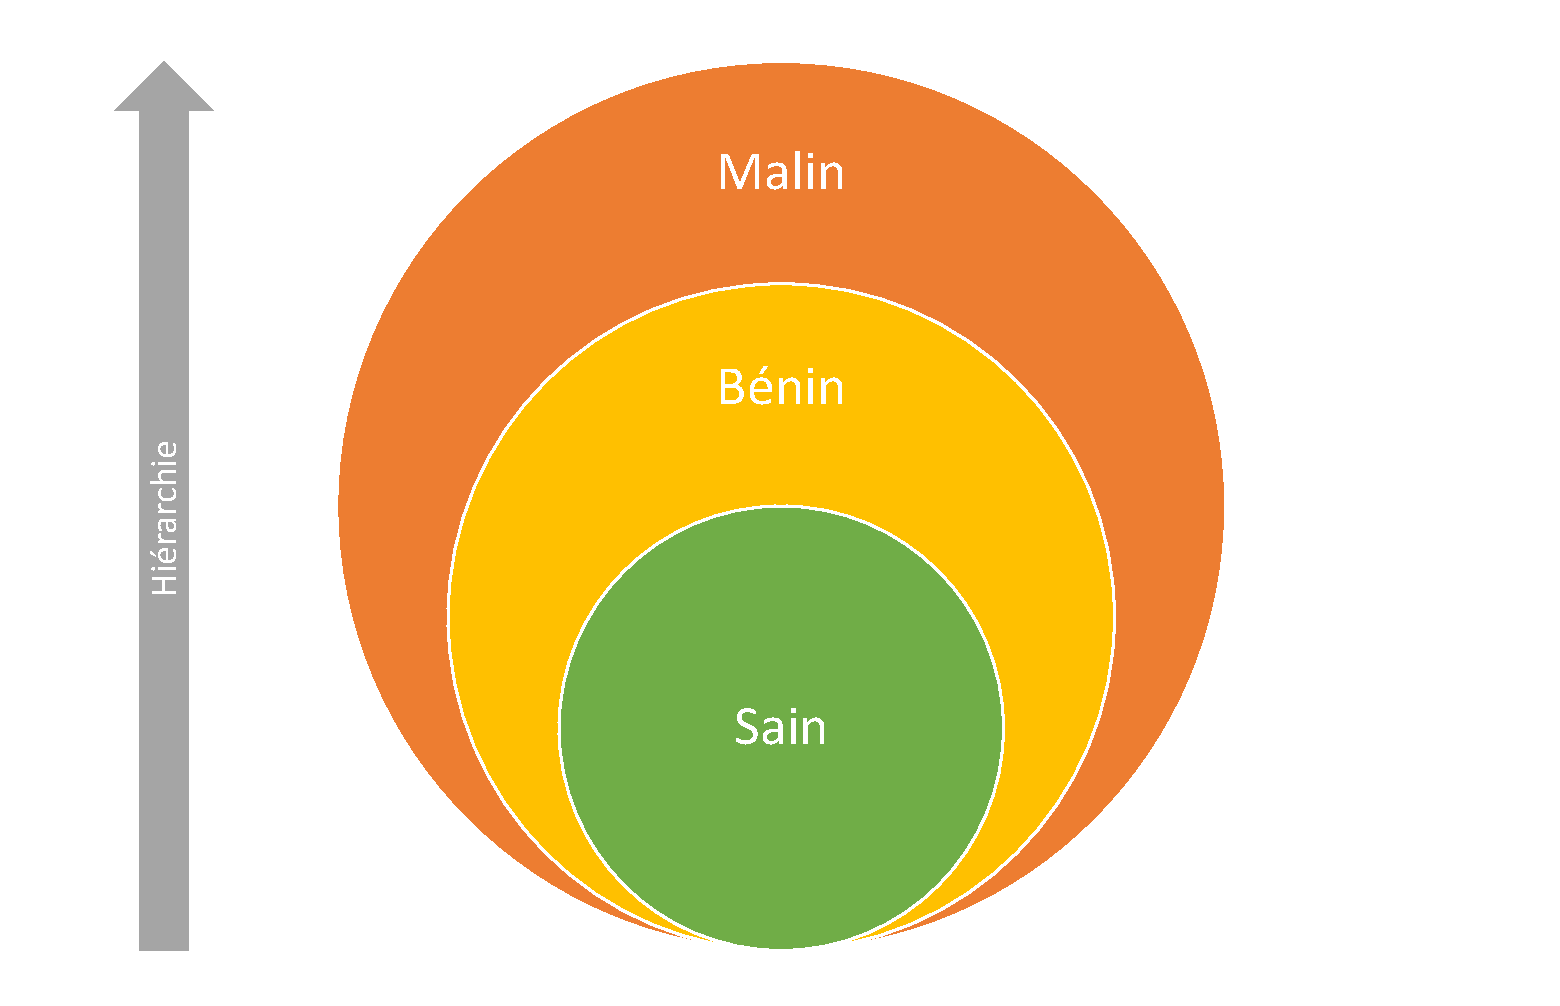
\includegraphics[width=0.7\textwidth]{contents/chapter_5/resources/scheme_annotations_hierarchy.pdf}
    \caption{Relation hiérarchiques entre les annotations. Les images malignes peuvent ainsi contenir des tissus bénin et sain ; Les images bénignes peuvent contenir des tissus sains ; Les images saines ne contiennent que des tissus sains.}
    \label{fig:scheme_annotations_hierarchy}
\end{figure}\par

Dans ce nouveau chapitre dédié à l'amélioration du diagnostic de l'image, nous exploiterons d'une part les conclusions du précèdent chapitre quant aux procédés de classification en privilégiant l'utilisation de \gls{svm} à noyau linéaire et d'autre part aux méthodes permettant l'extraction de l'information de texture. Ainsi, nous nous référerons aux méthodes suivantes :
\begin{itemize}
    \item pour la \textbf{catégorie de méthodes spatiales}, les caractéristiques définies par Haralick et al.,
    \item pour la \textbf{catégorie de méthodes spatiales}, les caractéristiques sur base d'extraction en ondelettes,
    \item pour la \textbf{catégorie de méthodes de transfert de connaissances}, nous utiliserons l'architecture ResNet.
\end{itemize}\par

Nous envisagerons de manière complémentaire des schémas alternatifs afin d'extraire une information suffisante à la séparation de nos données. Nous débuterons par la présentation de méthodes par multiples échelles, en supposant que l'information comporte plusieurs niveaux d'interprétations pouvant être capté par une méthode de classification. Dans un second temps, nous tenterons de capter l'information localement en employant un principe de fenêtres glissantes et de prédiction associées. Enfin, nous étendrons ces approches locales par l'utilisation de réseaux de \gls{cnn}, ajusté de bout en bout sur notre problème de classification à trois classes.\par
\clearpage

\section{Approche par échelles multiples}
Comme évoqué précédemment, les traitements réalisés jusqu'à lors ne permettent qu'une compréhension globale de l'image. Cette vision de l'extraction de caractéristiques peut être erronée si nous supposons une interprétation de l'image à divers niveaux de compréhension.\par

C'est ainsi que des hypothèses de compréhensions de l'image à multiples échelles ont émergées, bien que peu relatées dans la littérature. Ces approches ont été employées à différentes fins : 
\begin{inlinerate}
    \item de détection de frontières dans un contexte d'images naturelles~\cite{Ren2008},
    \item de segmentation d'images~\cite{Santos2012,Arbelaez2014},
    \item de détection d'objet~\cite{Felzenszwalb2008} ou d'actions~\cite{Pedersoli2011},
    \item ou encore de classification d'images médicales~\cite{Alsaih2016,Tang2017}.
\end{inlinerate} En termes d'images ~\gls{rcm} appliquée au domaine de la dermatologie, le travail de Wiltgen et al~\cite{Wiltgen2008} semble le plus proche et propose en autre le traitement de ces données par échelle multiples. Ainsi, nous scinderons cette section en deux parties respectives, avec d'une part l'application de ce principe à la décomposition en ondelettes et d'autres part l'application de ce principe à des techniques d'extraction spatiales.\par 

\subsection{Décomposition en ondelettes à échelles multiples}
Notre première approche par échelles multiples se portera sur la décomposition en ondelettes. En effet, ce principe a été démontré comme judicieux dans de nombreux domaines impliquant l'analyse d'images~\cite{Carvalho2004}. La décomposition peut ainsi être réalisé sous la forme d'un schéma dit diadique ou bien pyramidal. Ces deux mode sont schématisés sur la \Cref{fig:scheme_dwt_decomposition}. L'un de nos articles de référence préconise l'utilisation du schéma de décomposition diadique pour l'extraction de caractéristiques de texture sur images \gls{rcm}~\cite{Wiltgen2008}. Pour cela, cet article se focalise sur l'utilisation d'une ondelette mère de Daubechies et emploie la transformée en ondelette à cinq niveaux successifs sous forme d'arbre diadique. Les mesures associées à chaque bande de fréquences de la transformée sont les même que dans le \Cref{chap:chapter_4} et se base sur l'extraction de la déviation standard, l'énergie et l'entropie pour un total de \textbf{39 descripteurs}. Suite aux résultats obtenus lors du \Cref{chap:chapter_4}, nous évaluerons également ce procédé selon l'ondelette mère de Haar.\par

\begin{figure}[H]
    \centering
    \includegraphics[width=\textwidth]{contents/chapter_5/resources/scheme_dwt_decomposition.pdf}
    \caption{Schématisation deux principaux types de décomposition successives par ondelettes. En a), schéma de décomposition multi-échelle en ondelettes dit \textbf{diadique} ; En b), schéma de décomposition multi-échelle en ondelettes dit \textbf{pyramidal}.}
    \label{fig:scheme_dwt_decomposition}
\end{figure}\par

Le second travail sur base de décomposition en ondelettes sur lequel nous nous appuyons est une extension de la transformée en ondelettes du précédent travail~\cite{Halimi2017a}. Ainsi, ce travail reprend la précédente décomposition selon un schéma diadique, et modifie le nombre de niveaux de décomposition (quatre niveaux au lieu des cinq initialement prévu par Wiltgen et al.). Selon ce même travail, une loi normale généralisée centrée, dont la densité de probabilité $f$ est décrite par l'\Cref{eq:ggd}, est ajustée à la distribution de valeurs de chaque niveau de décomposition. Enfin, les auteurs de l'étude ne retiennent comme caractéristiques que les paramètres d'échelle $\alpha$ et de forme $\beta$ de cette loi normale généralisée pour un total de 24 caractéristiques.\par

\begin{equation}
    f(x)= \frac{\beta}{2\alpha\Gamma(1/\beta)} e^{-\left(|\frac{x}{\alpha}|\right)^\beta}
    \label{eq:ggd}
\end{equation}

Afin de gérer ces diverses caractéristiques, nous nous emploierons à l'utilisation d'un modèle de type \gls{svm} linéaire, démontré empiriquement efficace pour la classification de données fréquentielles dans ce contexte lors du \Cref{chap:chapter_4}. Les hyperparamètres que nous utiliserons pour validations sont présentés sur la \Cref{tab:image_improvement_multiscale_frequency}.\par

\begin{table}[H]
    \centering
    \begin{tabular}{cll}
        \toprule
        \textbf{Modèle}                                 & \textbf{Hyperparamètres}  & \textbf{Valeurs}                          \\ \midrule
        \gls{svm} - Noyau linéaire                      & C                         & [0.001, 0.01, 0.1, 1, 10, 100, 1000]      \\ 
        \bottomrule 
    \end{tabular} 
    \caption{Table reprenant le modèle et les hyperparamètres du modèle de classification employé pour la prédiction sur les caractéristiques fréquentielles par échelles multiples.}
    \label{tab:image_improvement_multiscale_frequency}
\end{table}\par

Nous effectuerons la transformée en ondelettes et la décomposition à échelles multiples de ce travail à l'aide de la bibliothèque logicielle "PyWavelets"~\cite{lee2006}. Quant aux opérations d'ajustement de la loi généralisée nous nous appuierons sur la bibliothèque logicielle "SciPy"~\cite{Virtanen2020}. L'ensemble de nos expérimentations basées sur la décomposition en ondelettes à échelle multiples sont recensées sur la \Cref{tab:wavelet_multiscale_nb_features} ainsi que leurs nombres de caractéristiques associées.\par

\begin{table}[h]
    \centering
    \begin{tabular}{ll}
        \toprule
        \textbf{Méthode}                                    & \textbf{Nombre de caractéristiques}   \\ \hline
        Ondelettes - Haar                                   & 39 (13$\times$3)   \\ \hline
        Ondelettes - Daubechies / Wiltgen~\cite{Wiltgen2008}& 39 (13$\times$3)   \\ \hline
        Halimi~\cite{Halimi2017a}                           & 24 (12$\times$2)   \\
        \bottomrule
    \end{tabular}
    \caption{Listes des méthodes sur base de décomposition par échelles multiples en ondelettes et leur nombre de caractéristiques extraites associées.}
    \label{tab:wavelet_multiscale_nb_features}
\end{table}\par

\subsection{Approche par échelles multiples}
Lors de la précédente sous-section, nous avons abordé les approches à échelle multiples sur base d'extraction en ondelettes. Toujours dans cette optique d'approche par échelle multiples, divers travaux se sont orientées afin de permettre une classification d'images médicale sur base d'extraction de caractéristiques spatiales~\cite{Alsaih2016,Tzalavra2016}. Les prochains étapes s'inspireront de ces travaux mais également des conclusions apportées par le \Cref{chap:chapter_4} sur l'extraction de caractéristiques spatiales et par transfert de connaissances. Ainsi, nous mettrons en œuvre deux processus par échelle multiples dans ce chapitre présentés lors des prochains paragraphes.\par

La première approche utilisée se base sur une approche de type fusion de caractéristiques avant l'étape de classification, telle qu'employé dans des travaux à but similaire~\cite{Pedersoli2011,Alsaih2016}. Afin de permettre l'agrégation des caractéristiques, nous emploierons un modèle \gls{svm} de type linéaire démontré efficace de manière empirique au sein du \Cref{chap:chapter_4} et robuste dans des contextes à forte dimensions. Les paramètres du modèle sont recensé sur la \Cref{tab:image_improvement_models_multiscale_spatial} et le principe de cette approche est schématisé au travers de la \Cref{fig:scheme_multiscale_features}.\par

\begin{figure}[H]
    \centering
    \includegraphics[width=\linewidth]{contents/chapter_5/resources/scheme_multiscale_features.pdf}
    \caption{Schéma de représentation du système par échelles multiple, sur la base d'une extraction à diverses échelles puis par l'agrégation des caractéristiques avant la procédure de classification.}
    \label{fig:scheme_multiscale_features}
\end{figure}\par

La seconde approche à échelles multiples correspond à un schéma en deux temps. En effet, nous considérerons dans cette seconde hypothèse la spécialisation de modèles de prédiction à des échelles précises. Nous emploierons à chacune de ces échelles, un modèle de type \gls{svm} linéaire pour les raisons évoquées précédemment, dont les hyperparamètres sont recensés en \Cref{tab:image_improvement_models_multiscale_spatial}. Pour cela, une étape d'entraînement de ces modèles sera réalisée en amont à l'aide de données d'entraînement accompagné par une étape de fusion des prédictions. Concernant la fusion de ces prédictions, le choix d'un vote à la majorité~\cite{Kam1994,Lam1997} a été évalué sur : 
\begin{inlinerate}
    \item les \textbf{décisions}, défini par l'ensemble $\mathbf{N}$,
    \item mais également sur les \textbf{scores}, défini par l'ensemble $\mathbf{R}$.
\end{inlinerate}
Il est à noter que ces schémas d'agrégation ne nécessitent aucune phase d'apprentissage. Afin de mettre en œuvre l'approche par scores, dans un premier temps, nous arborerons un schéma de type fonction de moyenne associé à la classe répertoriant le score le plus élevé. Ce schéma permet de notifier d'une tendance globale d'une classe par rapport aux autres. Dans un second temps, nous avons réalisé une approche de type fonction de maximum et détection de la classe recueillant le plus grand score. En effet, dans ce second schéma, nous optons pour une vision de la classe ayant recueilli la plus grande confiance. Le schéma global de cette expérience est présenté sur la \Cref{fig:scheme_multiscale_decision}.\par

\begin{figure}[H]
    \centering
    \includegraphics[width=\linewidth]{contents/chapter_5/resources/scheme_multiscale_decision.pdf}
    \caption{Schéma de représentation du système par échelles multiples, sur la base d'extraction d'extractions et de prédictions à diverses échelles et par agrégation de ces décisions.}
    \label{fig:scheme_multiscale_decision}
\end{figure}\par

\begin{table}[H]
    \centering
    \begin{tabular}{cll}
        \toprule
        \textbf{Modèle}                                 & \textbf{Hyperparamètres}  & \textbf{Valeurs}                          \\ \midrule
        \gls{svm} - Noyau linéaire                      & C                         & [0.001, 0.01, 0.1, 1, 10, 100, 1000]      \\ 
        \bottomrule 
    \end{tabular} 
    \caption{Table recensant les paramètres du modèle de classification employé pour réaliser la prédiction par échelles multiples sur caractéristiques spatiales ou par transfert de connaissances. Ce modèle et hyperparamètres sont employés pour la classification par échelle mais également pour l'agrégation des multiples échelles.}
    \label{tab:image_improvement_models_multiscale_spatial}
\end{table}\par

Ainsi, nous mènerons les diverses expériences de cette sous-section à l'aide des modes d'extraction précédemment étudié dans le \Cref{chap:chapter_4}. Nous emploierons dans un premier temps les caractéristiques d'Haralick~\cite{Haralick1973} extraites au nombre de 56 par image. Puis dans un second temps, le transfert de connaissances par l'utilisation de l'architecture de \gls{cnn} ResNett~\cite{He2016} pré-entrainé sur la base ImageNet~\cite{Canziani2016}, permettant l'extraction de 2048 d'entre elles par image. L'ensemble des expériences menées est recensé sur la \Cref{tab:spatial_transfer_multiscale_nb_features}.\par

\begin{table}[H]
    \centering
    \begin{tabular}{llll}
        \toprule
                                                    &          & \multicolumn{2}{l}{Nombre de caractéristiques} \\ \hline
        \multirow{2}{*}{Fusion de caractéristiques} & Haralick & \multicolumn{2}{l}{224 (56$\times$4)}          \\ \cline{2-4}
                                                    & ResNet   & \multicolumn{2}{l}{8192 (2048$\times$4)}       \\ \hline
        \multirow{2}{*}{Fusion de prédictions}      & Haralick & 56 / échelle   & \multirow{2}{*}{\begin{tabular}[c]{@{}l@{}}4 (1$\times$4) / Décisions\\ 12 (3$\times$4) / Scores\end{tabular}} \\ \cline{2-3}
                                                    & ResNet   & 2048 / échelle &                               \\
        \bottomrule
    \end{tabular}
    \caption{Listes des méthodes sur base de décomposition par échelles multiples et leur nombre de caractéristiques extraites associées.}
    \label{tab:spatial_transfer_multiscale_nb_features}
\end{table}\par


\section{Approche par fenêtre glissante}
Les hypothèses formulées lors du \Cref{chap:chapter_4} ne permettaient qu'une compréhension globale de l'image. Lors de la section précédente, nous avons évoqué des schémas par échelles multiples permettant une compréhension à divers niveaux. Cette nouvelle section va s'orienter vers une compréhension des données à basse échelle, en supposant qu'il existe un niveau de détail pour lesquels les tissus peuvent être caractérisés avec suffisamment de précision.\par

Ce type d'approche est souvent qualifié d'approche par fenêtres glissante ou par miniatures (termes anglais de \textit{patchs}). Néanmoins le premier terme permet de visualiser le principe de fonctionnement consistant à balayer un espace de plus grande dimension par une fenêtre de dimension inférieure. Cette technique a permis des avancées pour de diverses applications, dont : 
\begin{itemize}
    \item de la détection et localisation d'objets sur des images naturelles~\cite{Harzallah2009} ou encore de détection de cancer et de parties anatomiques sur image de radiologie~\cite{Helwan2017}, par motivation d'obtenir l'emplacement précis de certaines informations,
    \item de la détection d'anomalies sur des images histologiques mais encore de la classification de données conséquentes~\cite{Hou2016,Alqudah2019,Wei2019}, motivées par la contrainte matérielle impliqué par la taille de ces images ou par manque d'annotations,
    \item \ldots
\end{itemize}\par

Les données images en notre possession corroborent avec ce type de schéma, dans lequel chacune d'entre elle arbore une composition de tissus divers. Ces labels au niveau de l'image répondent à une hiérarchie mise en place pour qualifier les relations entre ces tissus. Pour rappel, un label malin qualifiera une donnée comportant au minimum des tissus typique d'une pathologie maligne mais pourra également comporter des tissus bénin et sain, et une annotation bénigne ne comportera que des tissus bénin ou sain.\par

Ce travail se distingue des travaux de Hou et al.~\cite{Hou2016} ou encore de Alqudah et al.~\cite{Alqudah2019} dans la mesure où nous possédons une base d'images de petite taille, soit 250$\times$250 pixels, annotée par l'un des spécialistes en dermatologie pour le besoin de cette étude. Cette taille a été déterminé car elle correspond a un bon compromis entre le niveau de détail et les tissus observables, mais également suite aux travaux de Wiltgen et al.\cite{Wiltgen2008} proposant des résultats en ce sens. Afin de nous affranchir partiellement de l'hypothèse de l'influence de la taille de la fenêtre glissante, nous proposerons une augmentation de ces images vers une taille de 500$\times$500 pixels, par mosaïquage, pour les expériences portant sur cette taille.\par

\begin{table}[H]
    \centering
    \begin{tabular}{cll}
        \toprule
        \textbf{Modèle}                                 & \textbf{Hyperparamètres}  & \textbf{Valeurs}                          \\ \midrule
        \gls{svm} - Noyau linéaire                      & C                         & [0.001, 0.01, 0.1, 1, 10, 100, 1000]      \\ 
        \bottomrule 
    \end{tabular} 
    \caption{Table reprenant le modèle et les hyperparamètres du modèle de classification employé pour la détection à basse échelle des tissus dans le processus de fenêtre glissante.}
    \label{tab:sliding_window_models}
\end{table}\par

Dans le but de mettre en oeuvre le schéma de détection à basse échelle, nous appliquerons les techniques jugées les plus pertinentes du chapitre précédent, à savoir : 
\begin{inlinerate}
    \item la méthode d'Haralick, comme représentant des méthodes spatiales,
    \item la méthode en ondelette de Daubechies, comme représentant des méthodes fréquentielles,
    \item et enfin une extraction selon l'architecture ResNet, comme représentant des méthodes par transfert de connaissances.
\end{inlinerate}. La détection à basse échelle sera réalisée à l'aide d'un modèle \gls{svm} linéaire, jugée le plus pertinent lors du \Cref{chap:chapter_4}, dont les paramètres sont listés en \Cref{tab:sliding_window_models}.\par

\begin{figure}[H]
    \centering
    \includegraphics[width=\linewidth]{contents/chapter_5/resources/scheme_sliding_features.pdf}
    \caption{Schéma de représentation du système de prédiction par fenêtre glissante. Ce schéma en deux temps propose de prédire sur une multitude de sous parties de l'image originale puis de fusionner les diverses prédictions afin de fournir une prédiction globale à la donnée originale.}
    \label{fig:scheme_sliding_features}
\end{figure}\par

Afin de gérer les prédictions obtenues au niveau de la fenêtre glissante, plusieurs stratégies sont envisagées sur les décisions et les scores. Ainsi, nous considérerons plusieurs approches, dont :
\begin{itemize}
    \item   une approche au niveau des \textbf{décisions}, défini par l'ensemble $\mathbf{N}$. Cette approche abouti à un vecteur de taille 1$\times$n où n correspond au nombre d'éléments extrait dans l'image. Deux méthodes ont été définies, dont : 
            \begin{itemize}
                \item par \textbf{priorité}, dans laquelle nous privilégions la détection d'un élément d'une classe hiérarchiquement supérieure comme décision globale à l'image,
                \item par seuils \textbf{dynamiques}, dans laquelle nous déterminons des seuils optimaux d'éléments nécessaires à chaque classe pour décréter l'appartenance à l'une d'entre elle, combiné à un système hiérarchique privilégiant les classes prioritaires.
            \end{itemize}
    \item   une approche au niveau des \textbf{scores}, défini par l'ensemble $\mathbf{R}$. Cette approche aboutie à un vecteur de taille s$\times$n où s correspond au nombre de scores de classes extrait et n correspond au nombre d'éléments extrait dans l'image. Deux méthodes ont été définies, dont : 
            \begin{itemize}
                \item par seuil \textbf{dynamique}, nous procédons dans un premier temps à une réduction de l'information à l'aide d'une fonction maximum, nous permettant de réduire celui-ci à vecteur de taille 1$\times$s focalisé sur la confiance maximum en chaque classe. Dans un second temps, des seuils optimaux représentant la confiance minimale nécessaire sont déterminé sur ces scores, combiné là encore à un système hiérarchique privilégiant les classes prioritaires.
                \item par \textbf{classification}, le vecteur de scores est alors considéré comme un vecteur de caractéristiques fourni en entrée d'un modèle \gls{svm} linéaire, dont les hyperparamètres considérés sont ceux de la \Cref{tab:sliding_window_models}.
            \end{itemize}
\end{itemize}\par

Nous n'envisagerons pas de scénario portant sur l'extraction de caractéristiques à l'aide la fenêtre de classification, c'est à dire sans l'étape de prédiction locale à chaque fenêtre, puis à la fusion de ces caractéristiques la dimension des données généré par une telle approche étant trop conséquente.\par
 
Nous emploierons pour cela un schéma de classification comme sur la \Cref{fig:scheme_sliding_features}. De plus, n'ayant pas de critères de tailles optimum, nous feront varier ces paramètres afin d'étudier leur impact sur la classification. ces paramètres sont visible sur la \Cref{tab:sliding_window_parameters}.\par

\begin{table}[H]
    \centering
    \begin{tabular*}{0.6\linewidth}{l@{\extracolsep{\fill}}l}
        \toprule
        \textbf{Résolution spatiale}& \textbf{Chevauchement}   \\ \hline
        250$\times$250              & 0\%                      \\ \hline
        250$\times$250              & 25\%                     \\ \hline
        250$\times$250              & 50\%                     \\ \hline 
        500$\times$500              & 0\%                      \\ \hline
        500$\times$500              & 25\%                     \\ \hline
        500$\times$500              & 50\%                     \\
        \bottomrule
    \end{tabular*}
    \caption{Ensemble des paramètres d'expérimentations menées par l'approche de type fenêtre glissante. Nous mesurerons ainsi l'impact de la résolution spatiale limité aux valeurs de 250$\times$250e t 500$\times$500, mais également du chevauchement sur des valeurs de 0\%, 25\% et 50\%.}
    \label{tab:sliding_window_parameters}
\end{table}\par

\section{Réglage fin de réseaux de convolution}
Dans cette partie, nous considérerons l'utilisation du réglage fin des \gls{cnn} adapté à notre problématique de classification d'images \gls{rcm}. En effet, cette méthode à été employée à des fins de détection de plans d'intérêts sur des images par ultrasons~\cite{Chen2015}, mais également de plans cardiaques sur des images d'\gls{mri}~\cite{Margeta2017}. Ce type d'approches a également été sollicité dans des approches semblables visant à de la détection de pathologies sur des acquisitions de rayons X réalisées sur des seins~\cite{Lotter2017} ou encore sur des poumons~\cite{Gao2018} avec des résultats très encourageants.\par

C'est donc de manière très naturelle que cette section s'oriente en ce sens, en se consacrant à ses divers aspects à l'aide de sous parties respectives propre à chaque concept. Nous débuterons par une présentation du réglage fin et du choix d'architecture considéré. Puis nous aborderons diverses techniques que nous mettrons en œuvre, dont :
\begin{inlinerate}
    \item l'augmentation de données,
    \item le programme d'apprentissage,
    \item et la fonction de coût.
\end{inlinerate}\par

\subsection{Présentation et mise en oeuvre de la méthode}
Le réglage fin est une extension de l'apprentissage par transfert dans laquelle sont substituées les couches de classification initiales du réseau par de nouvelles couches adaptée au problème. Cette approche se distingue dans la mesure où tout ou partie du réseau est réentraîné à partir des poids existants~\cite{Tajbakhsh2016}. Ce mode d'apprentissage est utilisé lorsque les données propres au nouveau problème sont suffisantes, et permet à l'instar du simple apprentissage par transfert d'obtenir un réseau plus adapté au problème cible. Néanmoins, ce mode d'apprentissage nécessite des ressources et un temps d'entraînement plus conséquent.\par

Afin de procéder à ce réglage fin, il est nécessaire de déterminer une architecture cible permettant de gérer au mieux la complexité des données. Par exemple un travail récent lors de la rédaction du manuscrit~\cite{Park2019} privilégie dans cette démarche l'utilisation d'une architecture ResNet-50~\cite{He2016} pour la détection de lésions pulmonaires sur des images de rayons X et propose la localisation de ces dernières. Néanmoins, aucune justification n'est apportée sur l'utilisation de cette architecture et aucune information n'est stipulée sur le type de Global Pooling employé par ce travail.\par

Lors du \Cref{chap:chapter_4} nous avons comparé les résultats des principales architectures de \gls{cnn} pre-éntrainés sur la base ImageNet, par application du principe d'apprentissage par transfert. Cette expérience nous a permis de déterminer de manière empirique que l'architecture de \gls{cnn} ResNet-50~\cite{He2016} est la plus adaptée en association à une couche de Global Pooling moyen. Ainsi, nous supposons que l'utilisation de l'architecture ResNet-50 et d'une couche de Global Pooling basé sur la moyenne, et couplé au principe du réglage fin est en mesure de spécialiser le réseau à la problématique de lésion de la peau sur images \gls{rcm}, et d'améliorer in fine ses performances.\par

Afin de procéder à la classification nous activation

Batch size / epoch / activation / learning rate

La fonction de coût est autre aspect que nous avons tenté de mener à bien dans ce travail.
~\cite{Park2019}
~\cite{Barbu2018}

Pour finir sur ces aspects de mise en oeuvre, nous précisons que l'ensemble de ces éléments ont été réalisées à haut niveau à l'aide de la bibliothèque logicielle "Keras"~\cite{chollet2015} compléméntairement à la bibliothèque de bas niveau "Tensorflow"~\cite{tensorflow2015}.\par

\subsection{Augmentation de données}
L'augmentation de données est une technique qui permet de corriger de manière artificielle le nombre d'exemples d'une base de données par application de transformations aux données d'origine~\cite{Wong2016,Taylor2018}. Ce type de méthode peut permettre de corriger un non-balancement des annotations, mais est essentiellement employé dans le but d'enrichir le nombre d'exemples disponible en aidant le réseau à focaliser sur des éléments essentiels à ceux-ci. Cela permet d'éviter qu'un réseau ne se focalise sur des éléments non essentiels à la tâche visée.\par

Nous envisageons dans cette sous-section cette technique comme le moyen d'enrichir notre base et ainsi d'éviter le sur-apprentissage potentiellement responsable de la dégradation des performances de prédiction. Les techniques considérées à cet effet ne correspondent uniquement qu'a des transformation géométriques linéaires~\cite{Taylor2018}, que nous opérerons de manière aléatoire à chaque étapes de l'entraînement(comprendre \textit{epochs}). Ces transformations ne sont appliquées que lors de l'entraînement, les images originales étant employées lors de l'évaluation. Les transformations considérées sont celles susceptibles de se produire dans un contexte clinique lors de l'acquisition des images, dont :
\begin{itemize}
    \item la rotation,
    \item la translation,
    \item ou encore la symétrie.
\end{itemize} De plus, nous opérerons à un repliement de l'information pour combler le vide généré par ces opérations, que nous jugerons plus "réaliste" sur les images que nous traitons qu'une unique valeur de remplissage.\par

Nous parlerons dans cette partie d'augmentation de données au sens de traitements appliqués au données d'entrées et non de création d'échantillons virtuels à partir de l'espace des caractéristiques pour corriger les problèmes de balancements~\cite{Wong2016}. Ainsi, nous considérerons l'augmentation de données comme une technique permettant de contrer le sur-apprentissage dans ce travail.\par

Ainsi, l'ensemble des paramètres appliqués à ces opérations sont décrit sur la \Cref{tab:image_improvement_data_augmentation}. Ces transformations sont appliquées aléatoirement et à la volée durant l'étape d'entraînement. Nous nous appuierons à cette fin sur le module d'augmentation de données de la bibliothèque logicielle "Keras"~\cite{chollet2015}.\par

\begin{table}[H]
    \centering
    \begin{tabular}{ll}
        \toprule
        \textbf{Nom}                            & \textbf{Valeurs}      \\ \midrule
        Rotation (en degrés)                    & [0 à 45]              \\ 
        Translation Horizontale (en pourcentage)& [0 à 20]              \\ 
        Translation Verticale (en pourcentage)  & [0 à 20]              \\  
        Symétrie Horizontale                    & [Désactivée,Activée]  \\  
        Symétrie Verticale                      & [Désactivée,Activée]  \\ 
        \bottomrule 
    \end{tabular} 
    \caption{Table recensant les paramètres de transformation appliqué aux données images de manière aléatoire lors de l'entraînement.}
    \label{tab:image_improvement_data_augmentation}
\end{table}\par

\subsection{Programme d'apprentissage}
Le programme d'apprentissage ou \textit{Curriculum Learning} est une démarche visant par analogie à l'humain, à entraîner tout \gls{cnn} en proposant diverses tâches intermédiaires avec une difficulté croissante, afin d'accomplir avec une plus grande efficacité une tâche plus complexe. La raison technique recherché par cette méthode est de simplifier l'espace de recherche de la tâche recherchée, afin de trouver plus efficacement un meilleur minimum au sein de la fonction de coût, comme suggéré par ses auteurs~\cite{Bengio2009}.\par

De récents travaux menés sur des images médicales, issue de rayons X, ont permis par cette approche d'augmenter les performance de détection de \gls{cnn} sur des cancer du sein~\cite{Lotter2017} ou encore des pathologies pulmonaires~\cite{Park2019}. La démarche suivie par ces deux travaux, est de procéder à l'extraction de sous images de taille restreinte autour des dites lésions avérées, en conservant la même propriété d'échelle que les images initiales. Cette extraction permet de réduire la résolution et la complexité du problème en proposant au réseau des images moins volumineuses et davantage focalisée sur des éléments clés afin d'éviter potentiellement des convergences non pertinentes. La gestion de donnée à échelles multiples sur \gls{cnn} ne donnant pas toujours lieu à des résultats suffisant~\cite{Noord2017}, une seconde étape d'entraînement est ensuite réalisée sur les images de taille réelles afin de former le réseau au problème que nous cherchons à résoudre.\par

En complément de cette technique, nous optons lors de la première phase de l'entraînement, à un entraînement en deux temps du réseau. En effet, l'ajout de couches connectées en fin de réseaux sous-entend une initialisation aléatoire de celui-ci. Ce phénomène peut conduire à une mauvaise remise en question de certain poids issus du caractère aléatoire de l'étape d'initialisation. Ainsi, nous procéderons à l'immobilisation des couches liés à l'extraction des caractéristiques dans un premier temps (pré-entraînement), puis à l'entraînement du réseau dans sa totalité. Le processus est schématisé sur la \Cref{fig:scheme_image_fine_tune}.\par

\begin{figure}[H]
    \centering
    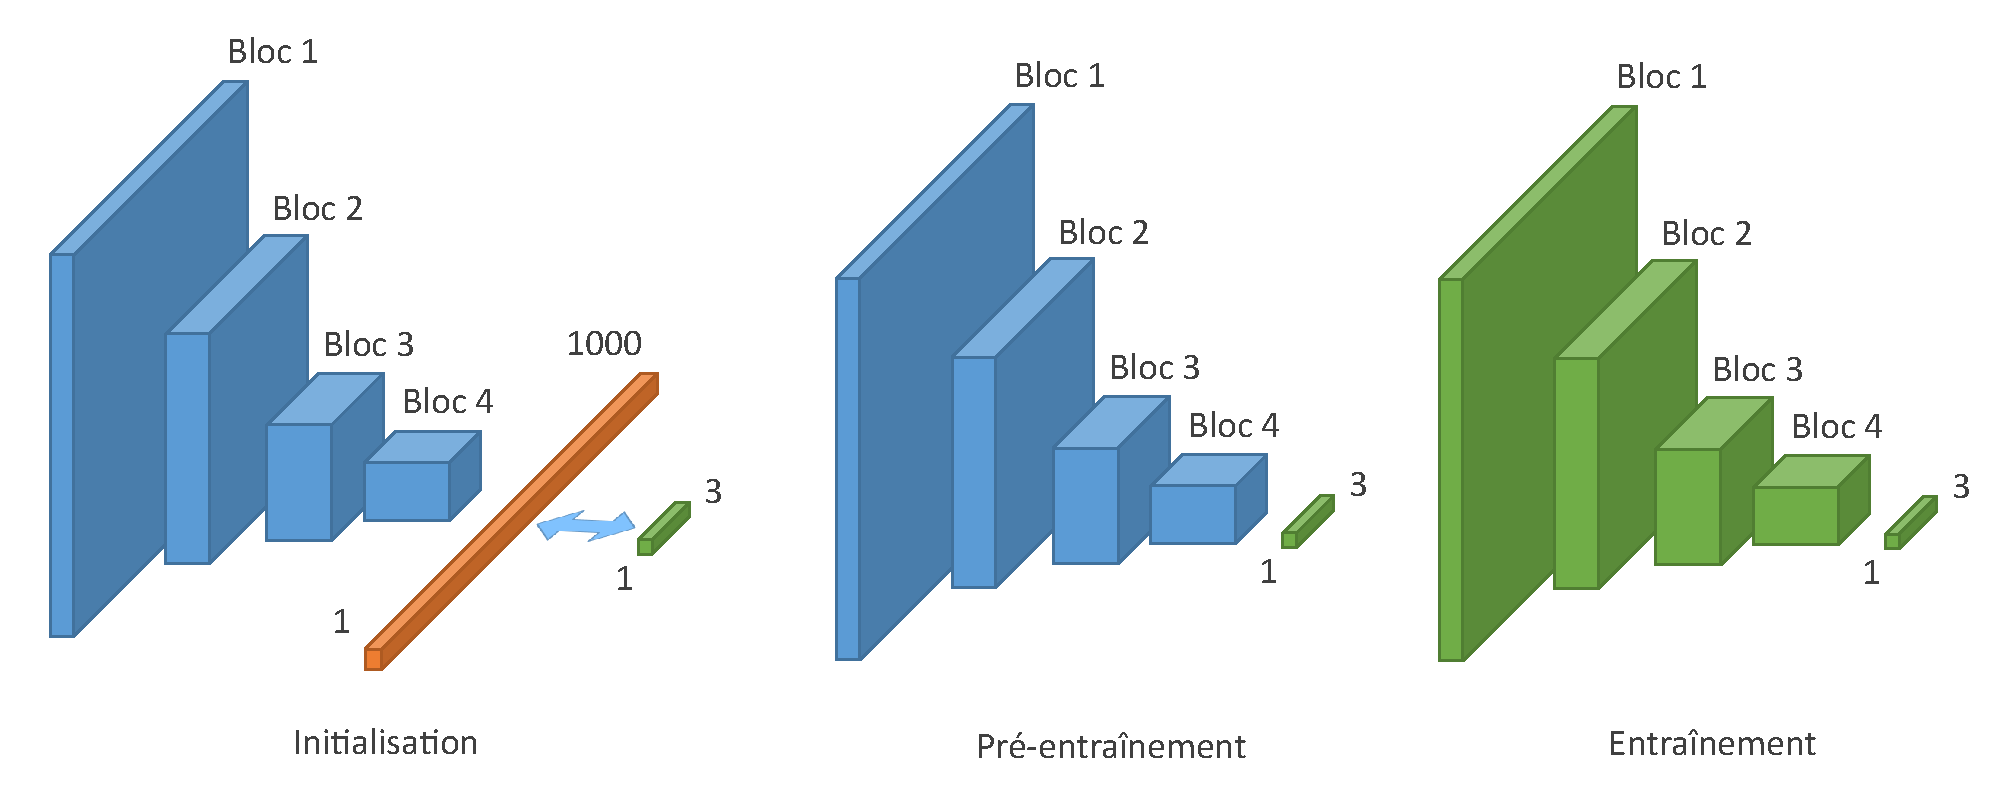
\includegraphics[width=\linewidth]{contents/chapter_5/resources/scheme_image_fine_tune.pdf}
    \caption{Schéma de représentation du processus de réglage fin utilisé dans ce travail. Celui-ci se décompose d'une étape d'initialisation dans le but de substituer les couches de classification par de nouvelles, puis un pré-entraînement permet d'initialiser les poids avant de procéder à l'entraînement.}
    \label{fig:scheme_image_fine_tune}
\end{figure}\par

\section{Analyse des résultats}

\begin{table}[H]
    \centering
    \begin{tabular}{llll}
        \toprule
        Catégories                  & Méthodes                  & 3 Classes         & Malin             \\ \midrule
        \multirow{3}{*}{Ondelettes} & Haar                      & 0.65±0.08         & 0.70±0.06         \\
                                    & Wiltgen~\cite{Wiltgen2008}& \textbf{0.66±0.06}& \textbf{0.71±0.06}\\
                                    & Halimi~\cite{Halimi2017a} & 0.38±0.02         & 0.41±0.04         \\ \midrule
        \multirow{5}{*}{Spatial}    & Fusion de caractéristiques& \textbf{0.63±0.06}& 0.66±0.07         \\
                                    & Décisions - Maximum       & 0.60±0.10         & 0.64±0.08         \\
                                    & Scores - Moyenne + Maximum& 0.60±0.10         & \textbf{0.67±0.07}\\
                                    & Scores - Maximum + Maximum& 0.59±0.10         & 0.65±0.08         \\
                                    & Scores - \gls{svm} Linéaire& 0.57±0.10        & 0.65±0.04         \\ \midrule
        \multirow{5}{*}{Transfert}  & Fusion de caractéristiques& \textbf{0.76±0.06}& \textbf{0.83±0.02}\\
                                    & Décisions - Maximum       & 0.69±0.10         & 0.78±0.05         \\
                                    & Scores - Moyenne + Maximum& 0.69±0.11         & 0.79±0.06         \\
                                    & Scores - Maximum + Maximum& 0.69±0.11         & 0.79±0.06         \\
                                    & Scores - \gls{svm} Linéaire& 0.72±0.04        & 0.79±0.03         \\
        \bottomrule
    \end{tabular}
    \label{tab:image_improvement_multiresolution}
    \caption{Résultats issus du processus de classification basé sur la classification multi-échelles.}
\end{table}


\begin{landscape}

\begin{table}[H]
    \centering
    \begin{tabular}{cclllllll}
		\toprule
		\multirow{2}{*}{Taille}     & \multirow{2}{*}{Superposition}    & \multirow{2}{*}{Mode}     & \multicolumn{2}{c}{Spatial}       & \multicolumn{2}{c}{Fréquence}     & \multicolumn{2}{c}{Transfert}         \\
		                            &                                   &                           & 3 Classes         & Malin         & 3 Classes         & Malin         & 3 Classes         & Malin             \\ \midrule
		250                         & Aucune                            & Patch                     & 0.67±0.10         & 0.41±0.13     & 0.72±0.07         & 0.44±0.10     & \textbf{0.91±0.02}& \textbf{0.82±0.03}\\ \midrule
		\multirow{12}{*}{250}       & \multirow{4}{*}{0}                & D\_ALO                    & 0.52±0.02         & 0.67±0.04     & 0.44±0.06         & 0.65±0.05     & 0.58±0.04         & 0.71±0.05         \\ 
							        &                                   & D\_DYN                    & 0.62±0.02         & 0.68±0.05     & 0.57±0.06         & 0.67±0.04     & 0.75±0.02         & 0.80±0.03         \\
							        &                                   & S\_MAX\_DYN               & 0.54±0.02         & 0.63±0.04     & 0.50±0.08         & 0.66±0.05     & 0.70±0.03         & 0.76±0.02         \\
							        &                                   & S\_SVC                    & 0.60±0.05         & 0.66±0.04     & 0.59±0.08         & 0.65±0.07     & 0.78±0.03         & 0.81±0.03         \\ \cline{2-9}
							        & \multirow{4}{*}{25}               & D\_ALO                    & 0.49±0.10         & 0.67±0.10     & 0.41±0.10         & 0.65±0.10     & 0.53±0.05         & 0.70±0.09         \\
							        &                                   & D\_DYN                    & 0.62±0.07         & 0.68±0.11     & 0.58±0.08         & 0.66±0.09     & 0.75±0.03         & 0.80±0.04         \\
							        &                                   & S\_MAX\_DYN               & 0.52±0.03         & 0.59±0.06     & 0.49±0.08         & 0.66±0.10     & 0.72±0.04         & 0.78±0.03         \\
							        &                                   & S\_SVC                    & 0.62±0.06         & 0.71±0.06     & 0.57±0.10         & 0.66±0.08     & 0.78±0.03         & 0.81±0.03         \\ \cline{2-9}
							        & \multirow{4}{*}{50}               & D\_ALO                    & 0.46±0.11         & 0.66±0.08     & 0.39±0.12         & 0.64±0.08     & 0.49±0.10         & 0.68±0.08         \\
							        &                                   & D\_DYN                    & 0.62±0.03         & 0.68±0.07     & 0.59±0.10         & 0.67±0.08     & 0.75±0.03         & 0.80±0.03         \\
							        &                                   & S\_MAX\_DYN               & 0.52±0.06         & 0.63±0.07     & 0.49±0.10         & 0.65±0.07     & 0.72±0.03         & 0.80±0.01         \\ 
		                            &                                   & S\_SVC                    & 0.61±0.08         & 0.69±0.08     & 0.61±0.07         & 0.68±0.06     & \textbf{0.78±0.03}& \textbf{0.82±0.02}\\ \midrule
		500                         & Aucune                            & Patch                     & 0.67±0.08         & 0.40±0.10     & 0.70±0.06         & 0.50±0.08     & \textbf{0.90±0.02}& \textbf{0.80±0.02}\\ \midrule
		\multirow{12}{*}{500}       & \multirow{4}{*}{0}                & D\_ALO                    & 0.58±0.08         & 0.63±0.05     & 0.23±0.11         & 0.00±0.00     & 0.74±0.05         & 0.76±0.05         \\
							        &                                   & D\_DYN                    & 0.59±0.04         & 0.63±0.05     & 0.28±0.05         & 0.63±0.05     & 0.72±0.05         & 0.76±0.05         \\
							        &                                   & S\_MAX\_DYN               & 0.50±0.05         & 0.56±0.15     & 0.53±0.08         & 0.66±0.04     & 0.70±0.03         & 0.78±0.04         \\
							        &                                   & S\_SVC                    & 0.59±0.08         & 0.67±0.07     & 0.36±0.04         & 0.55±0.17     & 0.69±0.13         & 0.74±0.08         \\ \cline{2-9}
							        & \multirow{4}{*}{25}               & D\_ALO                    & 0.55±0.08         & 0.64±0.07     & 0.23±0.11         & 0.00±0.00     & 0.77±0.05         & 0.80±0.04         \\
							        &                                   & D\_DYN                    & 0.55±0.10         & 0.63±0.05     & 0.28±0.05         & 0.63±0.05     & 0.76±0.04         & 0.80±0.04         \\
							        &                                   & S\_MAX\_DYN               & 0.53±0.03         & 0.55±0.09     & 0.54±0.07         & 0.67±0.05     & 0.73±0.03         & 0.80±0.04         \\
							        &                                   & S\_SVC                    & 0.58±0.07         & 0.67±0.06     & 0.37±0.04         & 0.55±0.18     & 0.77±0.05         & 0.81±0.04         \\ \cline{2-9}
							        & \multirow{4}{*}{50}               & D\_ALO                    & 0.57±0.08         & 0.67±0.11     & 0.23±0.07         & 0.00±0.00     & 0.77±0.03         & 0.81±0.05         \\
							        &                                   & D\_DYN                    & 0.58±0.07         & 0.67±0.11     & 0.28±0.12         & 0.63±0.12     & 0.76±0.03         & 0.80±0.05         \\
							        &                                   & S\_MAX\_DYN               & 0.52±0.05         & 0.55±0.06     & 0.55±0.07         & 0.67±0.13     & 0.73±0.04         & 0.80±0.05         \\
		                            &                                   & S\_SVC                    & 0.60±0.06         & 0.65±0.09     & 0.34±0.05         & 0.39±0.23     & \textbf{0.78±0.02}& \textbf{0.81±0.04}\\
		\bottomrule
    \end{tabular}
    \label{tab:image_improvement_sliding_window}
    \caption{Résultats issus du processus de classification basé sur les fenêtres glissantes. La première partie reprend les résultats obtenu à l'aide d'un classifieur et d'une fenêtre glissante d'une taille de 250 par 250 pixels ; La seconde partie  reprend les résultats obtenu à l'aide d'un classifieur et d'une fenêtre glissante d'une taille de 500 par 500 pixels.}
\end{table}

\end{landscape}

\begin{table}[H]
    \centering
    \begin{tabular}{llll}
        \toprule
        Catégorie                   & Pooling           & 3 Classes         & Malin             \\ \midrule
        \multirow{2}{*}{Réglage fin}& Fonction moyenne  & 0.44±0.05         & 0.69±0.06         \\
                                    & Fonction maximum  & \textbf{0.56±0.05}& \textbf{0.78±0.05}\\
        Réglage fin + Programme     & Fonction maximum  & 0.51±0.07         & 0.67±0.05         \\
        \bottomrule
    \end{tabular}
    
    \label{tab:image_improvement_fine}
    \caption{Résultats issus du processus de classification basé sur les \gls{cnn} par réglages fin et programme d'apprentissage.}
\end{table}

Nous finirons cette section dédiée aux résultats par la proposition d'extensions aux principes de fenêtre glissante mais aussi de réglage fin de \gls{cnn}. En effet, ces deux techniques possèdent par leur nature la capacité de localiser précisément l'origine d'une information. Dans le cadre des fenêtres glissantes, c'est de manière directe que ce principe permet de remonter l'emplacement d'une décision, nous proposons ainsi deux modes de visualisation l'un basé sur les décisions en utilisant un code couleur propre à chacune ou sur les scores en utilisant l'intensité de la transparence comme indicateur dans la confiance de la prédiction. Ces deux propositions sont visibles sur la \Cref{fig:exemple_image_improvement_well} et la \Cref{fig:exemple_image_improvement_misclassified}. Ainsi, une taille de fenêtre glissante la plus fine permettra par cette technique d'obtenir une information visuelle de meilleure qualité, dualité que nous pouvons observer entre les tailles de 250$\times$250 et 500$\times$500.\par

\begin{figure}[H]
    \centering
    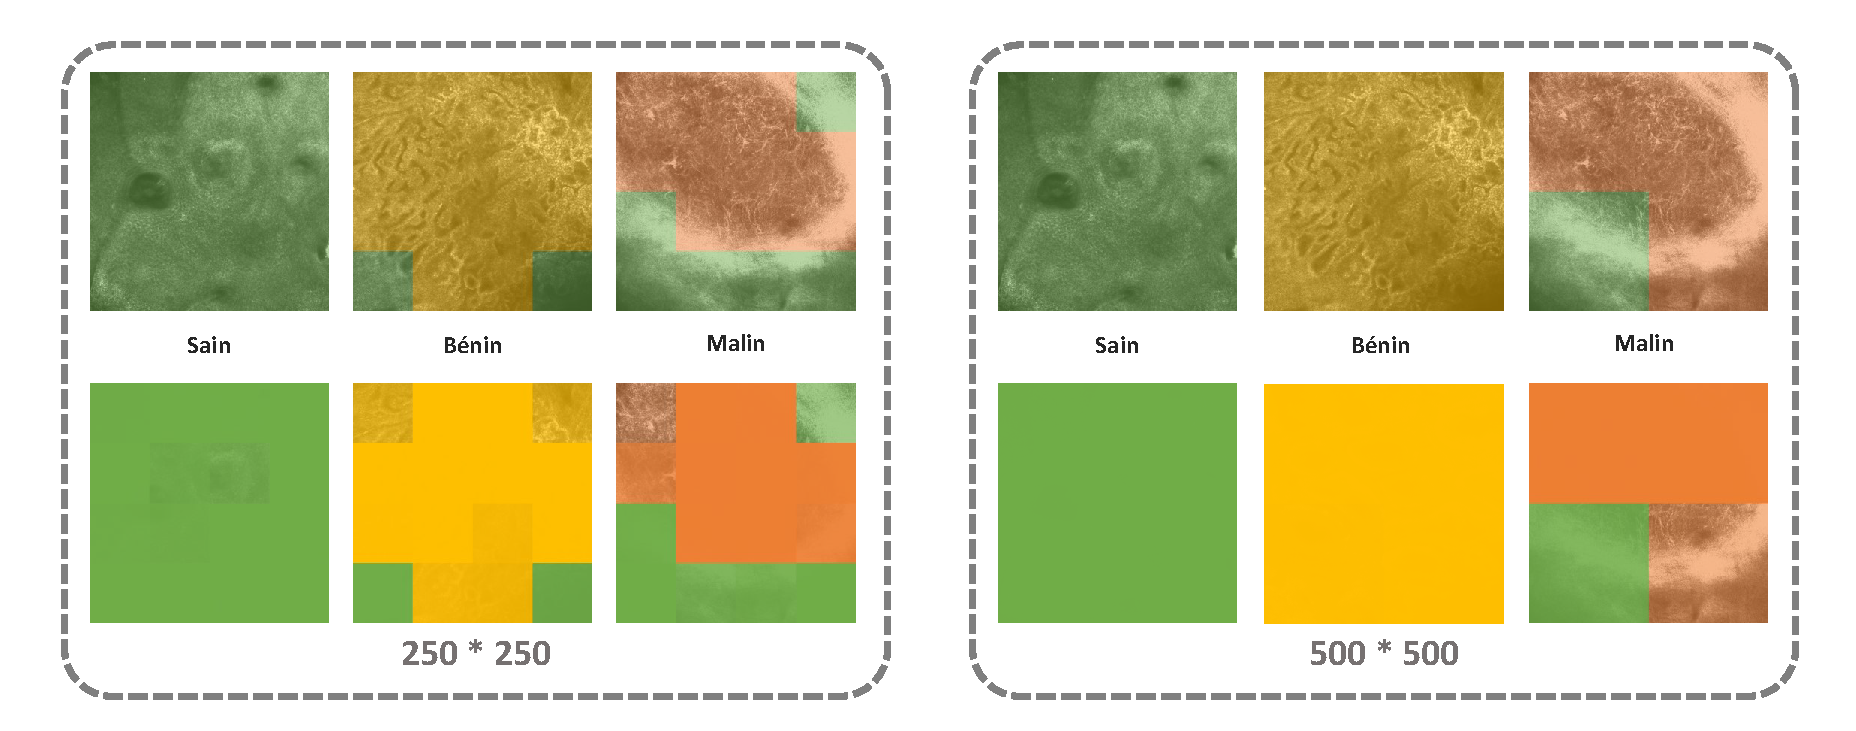
\includegraphics[width=\linewidth]{contents/chapter_5/resources/exemple_image_improvement_well.pdf}
    \caption{Exemple d'image correctement classifiées à l'aide du principe de fenêtre glissante. A gauche, résultats issus d'une fenêtre de classification de 250 par 250 pixels ; A droite, résultats issu d'une fenêtre de classification de 500 par 500 pixels.}
    \label{fig:exemple_image_improvement_well}
\end{figure}\par

\begin{figure}[H]
    \centering
    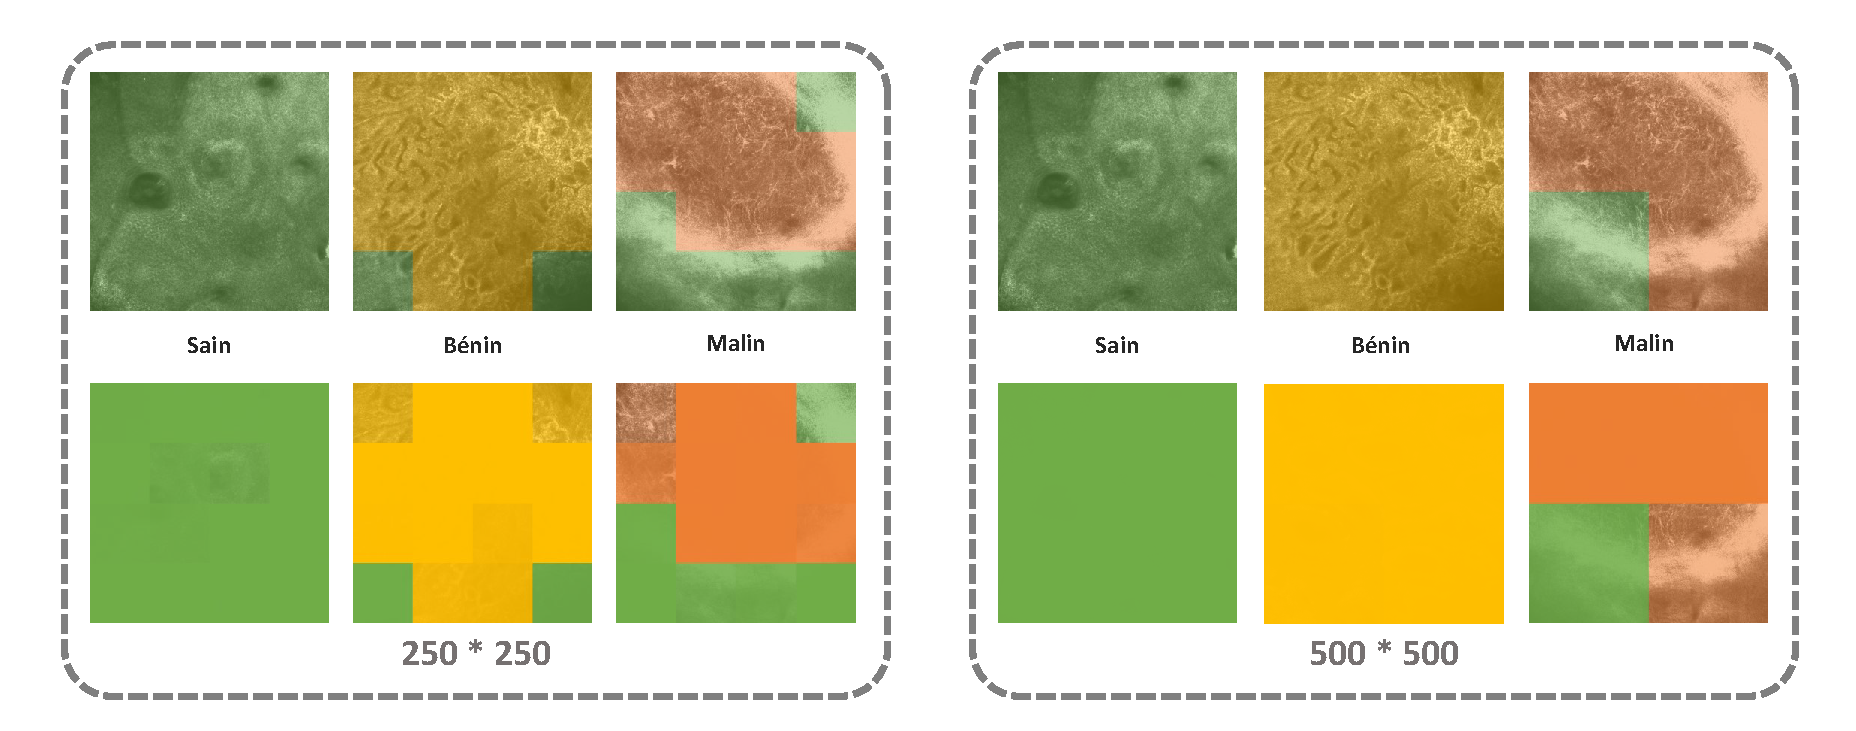
\includegraphics[width=\linewidth]{contents/chapter_5/resources/exemple_image_improvement_well.pdf}
    \caption{Exemple d'image incorrectement classifiées à l'aide du principe de fenêtre glissante. A gauche, résultats issus d'une fenêtre de classification de 250 par 250 pixels ; A droite, résultats issu d'une fenêtre de classification de 500 par 500 pixels.}
    \label{fig:exemple_image_improvement_misclassified}
\end{figure}\par


~\cite{jia2017}
\begin{figure}[H]
    \centering
    \includegraphics[width=\linewidth]{contents/chapter_5/resources/exemple_image_improvement_activation_maps.pdf}
    \caption{Exemple d'image .}
    \label{fig:exemple_image_improvement_activation_maps}
\end{figure}\par